\documentclass[12pt,oneside,a4paper,semicolon]{book} % This style for A4 format. 
\usepackage{amsmath, amssymb, amsthm}
\usepackage{graphicx,color}
\usepackage{multirow}
\usepackage[left=1.5in, right=1in, top=1in, bottom=1in]{geometry}
\usepackage{float}
\usepackage{epsfig}
\usepackage{color}
%For Terms and Abbreviations 
%\usepackage{glossaries}
\usepackage[acronym,toc=true,section=section, nogroupskip,nonumberlist]{glossaries}
\makeglossaries
\renewcommand*\glspostdescription{\cftdotfill{\cftsecdotsep}}
%\renewcommand{\glossarysection}[2][]{{\centering\bfseries\MakeTextUppercase{#2}\par}}



\usepackage{ragged2e}
\usepackage[dvipsnames]{xcolor}
\usepackage{setspace}
\usepackage{latexsym}
\usepackage{mathrsfs}
\usepackage{graphicx}
\usepackage{tikz}
\usepackage[titletoc]{appendix}
\usepackage{alltt}
\graphicspath{ {images/} }
\usepackage{longtable}
\usepackage{tikz}
\usepackage{acronym}
\usepackage{pgfplots}
\pgfplotsset{compat=1.18}
\usepackage{csquotes}
\usepackage[hidelinks]{hyperref}
%\usepackage{tocloft}
\setcounter{tocdepth}{2}
%\renewcommand{\cftdot}{}
\usepackage{titletoc,tocloft}
\setlength{\cftchapnumwidth}{1cm} % Adjust chapter number width (optional)
\setlength{\cftsecindent}{1cm}   % Set section indent to 1cm
\setlength{\cftsubsecindent}{1.5cm}  % Set subsection indent to 1.5cm
%\dottedcontents{section}[1.5em]{}{1.3em}{.6em}


\usepackage{times}
\renewcommand{\baselinestretch}{1.25}
\usepackage{sectsty}
\usepackage{titlesec}
\usepackage[T1]{fontenc}
\setcounter{secnumdepth}{3}
\chapterfont{\centering }
\titleformat{\chapter}[display]
{\normalfont%
	\huge% %change this size to your needs for the first line
	\bfseries}{\chaptertitlename\ \thechapter}{16pt}{%
	\Huge %change this size to your needs for the second line
}
%{\bf\centering }
%{\chaptertitlename\ \thechapter }{14pt}{\large}

\usepackage{textcase}
%\allsectionsfont{\MakeTextUppercase}

\sectionfont{\normalfont}
\titleformat{\section}
%\renewcommand{\section}[1]{\bfseries\section}
{\normalfont\fontsize{14pt}{16pt} \bfseries \selectfont}{ \thesection}{1em}{}
\titleformat{\subsection}
{\normalfont\fontsize{12pt}{14pt} \selectfont}{\thesubsection}{1em}{}
\titleformat{\subsubsection}
{\normalfont\fontsize{12pt}{14pt} \selectfont}{\thesubsubsection}{1em}{}
\titlespacing*{\section} {0pt}{0pt}{2.3ex plus .2ex}
\titlespacing*{\subsection}{0pt}{0pt}{1.5ex plus .2ex}
%\titlespacing*{\section} {0pt}{0pt}{2.3ex plus .2ex}
%\titlespacing*{\subsection}{0pt}{0pt}{1.5ex plus .2ex}
\usepackage{caption}
\captionsetup[table]{labelsep=space,labelfont=bf,font=footnotesize} 
\captionsetup [figure]{labelsep=space,labelfont=bf,font=footnotesize}
\setcounter{page}{1}
\newtheorem{definition}{Definition}
\newcommand{\brdefinition}{\begin{definition}}
	\newcommand{\erdefinition}{\end{definition}}

\newtheorem{corollary}{Corollary}
\newcommand{\bcorollary}{\begin{corollary}}
	\newcommand{\ecorollary}{\end{corollary}}
\newtheorem{example}{Example}
\newcommand{\bexample}{\begin{example}}
	\newcommand{\eexample}{\end{example}}
\newtheorem{remark}{Remark}
\newcommand{\bremark}{\begin{remark}}
	\newcommand{\eremark}{\end{remark}}
\newcommand{\bproof}{{\bf {Proof:}}}
\newcommand{\eproof}{}
\newcommand{\bsolution}{{\bf {Solution:}}}
\newcommand{\esolution}{}
\newtheorem{theorem}{Theorem}
\newcommand{\btheorem}{\begin{theorem}}
	\newcommand{\etheorem}{\end{theorem}}
\newtheorem{lemma}{Lemma}
\newcommand{\blemma}{\begin{lemma}}
	\newcommand{\elemma}{\end{lemma}}
\newcommand{\UD}{\ensuremath{\bigtriangleup}}
\newcommand{\IC}{\ensuremath{\mathcal{C}} }
%\renewcommand{\rm}{\normalshape}
\newcommand{\ol}{\overline}
\def\cen{\centerline}
\def\pnq{\par\noindent\quad}
\def\pn{\par\noindent}
\newcommand{\non}{\nonumber}
\newcommand{\mC}{{\mathbb C}}
\newcommand{\mN}{{\mathbb N}}
\newcommand{\mU}{{\mathbb U}}
\newcommand{\cA}{{\mathcal A}}
\newcommand{\cR}{{\mathcal R}}
\newcommand{\cS}{{\mathcal S}}
\newcommand{\cT}{{\mathcal T}}
\newcommand{\cUCV}{{\mathcal UCV}}
\newcommand{\cST}{{\mathcal ST}}
\newcommand{\cK}{{\mathcal K}}
\newcommand{\ds}{\displaystyle}
\newcommand{\brdef}{\begin{defi}}
	\newcommand{\erdef}{\end{defi}}
\newcommand{\bcor}{\begin{cor}}
	\newcommand{\ecor}{\end{cor}}
\newcommand{\bth}{\begin{thm}}
	\newcommand{\ble}{\begin{lem}}
		\newcommand{\ele}{\end{lem}}
	\newcommand{\bcha}{\end{cha}}\pagestyle{plain}
\renewcommand{\theequation}{\thechapter.\arabic{equation}}
\renewcommand{\thetheorem}{\thesection.\arabic{theorem}}
\renewcommand{\thecorollary}{\thesection.\arabic{corollary}}
\renewcommand{\thelemma}{\thesection.\arabic{lemma}}
\renewcommand{\thedefinition}{\thesection.\arabic{definition}}
\renewcommand{\theexample}{\thesection.\arabic{example}}
\renewcommand{\theremark}{\thesection.\arabic{remark}}
\renewcommand{\thechapter}{\arabic{chapter}}
\renewcommand{\thesection}{\thechapter.\arabic{section}}

%\renewcommand{\&}{and}
\renewcommand{\chaptername}{CHAPTER}
\renewcommand{\figurename}{Fig.}

\def\cen{\centerline}
\def\pnq{\par\noindent\quad}
\def\pn{\par\noindent}
\def\sevenpoint{%
	\def\rm{\sevenrm}%
	\def\it{\sevenit}%
	\def\bf{\sevenbf}%
	\rm}
%\pretoler
\renewcommand{\theequation}{\thechapter.\arabic{equation}}
\theoremstyle{definition}
\renewcommand*{\proofname}{{\rm Proof}}
%%%%%%%%%%%%%%%%%%%%%%%%%%%%%%%%%%%%%%%%%%%%%%%%%%%%%%%%%%%%%%%%%%%Chapter title format
\usepackage{sectsty}
\usepackage{titlesec}
\chapterfont{\centering }
\titleformat{\chapter}[display]
{\bf\centering}
{\chaptertitlename\ \thechapter}{16pt}{\large}
\sectionfont{\normalfont}
%\renewcommand*\contentsname{\large \centerline{TABLE OF CONTENTS}}
%\renewcommand\cftchappresnum{} % prefix "Chapter " to chapter number in ToC
%\cftsetindents{chapter}{0em}{3em}      % set amount of indenting
%\cftsetindents{section}{0em}{3em}
%For reference

%\usepackage{natbib}
%\bibliographystyle{apalike}%\usepackage{apalike}
%\setcitestyle{square}
%\setlength{\bibhang}{0pt}

% ******* References config *********
\bibliographystyle{IEEEtran}   % On some TeX systems this works
%\bibliographystyle{ieeetr}      % While on others this works
							% Uncomment and test if your references don't cite
							% correctly
\renewcommand{\bibname}{References}
%\setlength\bibindent{0em}
%\renewcommand{\bibname}{REFERENCES}
%\renewcommand{\bibname}{\protect\centerline{References}}

%\newcommand{\setbibname}[1]{\bibname[#1]{\centering #1}}


\renewcommand*\contentsname {\large \centerline{TABLE OF CONTENTS}}
\renewcommand*\listfigurename{ \large \centerline{{LIST OF FIGURES}}}
\renewcommand*\listtablename{ \large \centerline{{LIST OF TABLES}}}


\usepackage{datetime}
\newdateformat{monthyeardate}{%
  \monthname[\THEMONTH], \THEYEAR}
%\renewcommand*{\bibpagespunct}{\addcolon\space}

\definecolor{butter1}{rgb}{0.988,0.914,0.310}
\definecolor{chocolate1}{rgb}{0.914,0.725,0.431}
\definecolor{chameleon1}{rgb}{0.541,0.886,0.204}
\definecolor{skyblue1}{rgb}{0.447,0.624,0.812}
\definecolor{plum1}{rgb}{0.678,0.498,0.659}
\definecolor{scarletred1}{rgb}{0.937,0.161,0.161}

\usepackage{listings}
\usepackage{color}

\definecolor{dkgreen}{rgb}{0,0.6,0}
\definecolor{gray}{rgb}{0.5,0.5,0.5}
\definecolor{mauve}{rgb}{0.58,0,0.82}
%language options
%C/C++
%Python
%Ruby
%Perl
%PHP
%JavaScript
%HTML
%XML
%SQL
\lstset{frame=tb,
  language=Python,
  aboveskip=3mm,
  belowskip=3mm,
  showstringspaces=false,
  columns=flexible,
  basicstyle={\small\ttfamily},
  numbers=none,
  numberstyle=\tiny\color{gray},
  keywordstyle=\color{blue},
  commentstyle=\color{dkgreen},
  stringstyle=\color{mauve},
  breaklines=true,
  breakatwhitespace=true,
  tabsize=3
}


%For Table Column Width
\usepackage{array}
\newcolumntype{L}[1]{>{\raggedright\let\newline\\\arraybackslash\hspace{0pt}}m{#1}}
\newcolumntype{C}[1]{>{\centering\let\newline\\\arraybackslash\hspace{0pt}}m{#1}}
\newcolumntype{R}[1]{>{\raggedleft\let\newline\\\arraybackslash\hspace{0pt}}m{#1}}

\usepackage{etoolbox}

\makeatletter
\patchcmd{\ttlh@hang}{\parindent\z@}{\parindent\z@\leavevmode}{}{}
\patchcmd{\ttlh@hang}{\noindent}{}{}{}
\makeatother



\begin{document}

\onehalfspacing
\thispagestyle{empty}

%{\textit{Synopsis of the Thesis}}
\centering
\textcolor{Cyan}{\large \textbf{A Project Report}} \\
\begin{center}
    on\\
\end{center}
\begin{spacing}{1.5}
    

 \textcolor{ForestGreen}{\MakeUppercase{\Large \textbf{Your Title here}}}

 \textcolor{Red}{submitted in partial fulfillment of the requirements for the award of the degree of} 
\end{spacing}
\begin{center}
    
\vskip 0.2cm
\textcolor{Orange}{{\large \textbf{BACHELOR OF TECHNOLOGY\\
in\\
COMPUTER SCIENCE \& ENGINEERING\\}}}
\end{center}
\vskip .2cm
\begin{center}
  \textcolor{violet}{   \textbf{by}}
\end{center}
\vskip .2cm

\begin{center}
 \textbf{\textcolor{violet}{   \begin{tabular}{cc}
  \MakeUppercase{21wh1a0588}   &  \MakeUppercase{xyz}\\
   \MakeUppercase{21wh1a0588}   &  \MakeUppercase{xyz}\\
    \MakeUppercase{21wh1a0588}   &  \MakeUppercase{xyz}\\
\end{tabular}}}
\end{center}
% {\Large \textbf {of}}
% \vskip .2cm
% {\Large \textbf {Everything}}
\vskip 0.2cm
\begin{spacing}{1.25}
    \begin{center}
    \textbf{
    Under the esteemed guidance of\\
\large{Dr. \MakeUppercase{Venkatesh B}}\\
Associate Professor\\
    }
\end{center}
\end{spacing}

\centerline{
\includegraphics[scale=1.5]{bvrit}}
\vskip 0.5cm
\begin{center}
    \textbf{
  \textcolor{Bittersweet}{\Large Department of Computer Science \& Engineering} \\
  \vskip 0.2cm
  \textcolor{RoyalPurple}{\large\MakeUppercase{BVRIT HYDERABAD COLLEGE OF ENGINEERING FOR WOMEN}\\
  \vskip 0.2cm
\normalsize (NAAC Accredited-A Grade | NBA Accredited B.Tech (EEE, ECE, CSE, and IT))\\
(Approved by AICTE, New Delhi and Affiliated to JNTUH, Hyderabad)\\
Bachupally, Hyderabad – 500090\\}
\monthyeardate\today
    }
\end{center}



\newpage
\begin{spacing}{1.5}

\begin{center}
    \textbf{
  \textcolor{RoyalPurple}{\Large BVRIT HYDERABAD\\
COLLEGE OF ENGINEERING FOR WOMEN\\
\normalsize (NAAC Accredited-A Grade | NBA Accredited B.Tech (EEE, ECE, CSE, and IT))\\
(Approved by AICTE, New Delhi and Affiliated to JNTUH, Hyderabad)\\
Bachupally, Hyderabad – 500090\\}
\vskip 0.5cm
  \textcolor{Bittersweet}{\Large Department of Computer Science \& Engineering} \\
}
\end{center}




\begin{center}
\thispagestyle{empty}
\vskip .5cm
\centerline{
\includegraphics[scale=1.25]{bvrit}}
\vskip .3cm
{\centerline{ {\large \textbf{CERTIFICATE}}}}
\end{center}
\justifying
This is to certify that the Project Work report on “\textbf{\MakeUppercase{facial emotion recognition using deep learning model}}” is a bonafide work carried out by \textbf{Ms. P. Sridevi
(\MakeUppercase{20WH1A05E4}), Ms. N. Sai Manogna (\MakeUppercase{20WH1A05E4}), and Ms. N. Sai Manogna (\MakeUppercase{20WH1A05E4})} in the partial fulfillment for the
award of B.Tech. degree in \textbf{Computer Science \& Engineering}, \textbf{BVRIT HYDERABAD
College of Engineering for Women}, Bachupally, Hyderabad, affiliated to Jawaharlal Nehru
Technological University Hyderabad, Hyderabad under my guidance and supervision. The
results embodied in the project work have not been submitted to any other University or
Institute for the award of any degree or diploma.\\
~\\

\noindent
\begin{minipage}{10cm}
 \textbf{Internal Guide}\\
Dr. Venkatesh B\\ 
Associate Professor\\
Department of CSE
\end{minipage}
\begin{minipage}{10cm}
   \textbf{Head of the Department}\\
Dr. M Sreevani\\
Professor\\
Department of CSE
\end{minipage}

\vskip 2cm
\begin{center}
  \textbf{External Examiner}  
\end{center}

					  	


\newpage
\begin{center}
\thispagestyle{empty}
%{\textbf{\textit{SYNOPSIS OF}}}
\vskip .5cm
{\centerline {{\large \textbf{DECLARATION}}}}
\end{center}

% {\Large \textbf {An Overview}}
% \vskip .2cm
% {\Large \textbf {of}}
% \vskip .2cm
% {\Large \textbf {Everything}}

\par \quad \quad We hereby declare that the work presented in this project entitled \textbf{\enquote {\MakeUppercase{Title}}} submitted towards
completion of Project Work in IV year of B.Tech., CSE at ‘BVRIT HYDERABAD College
of Engineering for Women’, Hyderabad is an authentic record of our original work carried
out under the guidance of \textbf{Dr. Venkatesh B},
Associate Professor, Department of CSE.

~\\

\noindent
\begin{minipage}{10cm}
~\\
% \textbf{Internal Guide}\\
%Dr. R. Suneetha Rani\\ 
%Designation\\
%Department of CSE
\end{minipage}
\begin{minipage}{20cm}
\vskip 1cm
  \textbf{Student Name}\\
  \textbf{(Roll No)}
\vskip 2cm
    \textbf{Student Name}\\
  \textbf{(Roll No)}

  \vskip 2cm
    \textbf{Student Name}\\
  \textbf{(Roll No)}

 % \vskip 2cm
 %   \textbf{Student Name}\\
 % \textbf{(Roll No)}
\end{minipage}
\newpage
\pagenumbering{roman}
%\begin{center}
%\large\textbf{ABSTRACT} 
%\end{center}
%\vspace*{1cm}
%\chapter*{\centering \underline{\large\textbf{ABSTRACT}}}
%\addcontentsline{toc}{chapter}{\bf ~~~~~~~~~~ABSTRACT}
\addcontentsline{toc}{section}{\bf ABSTRACT}
{\centerline { {\large \textbf{ABSTRACT}}}}
~\\

The abstract should be one page synopsis of the thesis typed one and a half line spacing, Font Style: Times New Roman and Font Size: 12.  The abstract is a very brief summary of the thesis contents. It should be about one page long not more than 300 words.  The 300-word statement should describe the problem addressed by your thesis, a description of the work completed and a summary of any findings or lessons learned. The format is given in Appendix D.
     
\vskip 0.5cm
\noindent
\textbf{Keywords:} {\it Thesis}, {\it Dissertation}, {\it Degree}, {\it Sample Thesis}, {\it Literature}.  

\newpage
%\begin{center}
%\underline{\large\textbf{ACKNOWLEDGEMENT}} 
%\end{center}
%\addcontentsline{toc}{section}{\bf ACKNOWLEDGMENT}
{\centerline { {\large \textbf{ACKNOWLEDGMENT}}}}
\thispagestyle{empty}
\vspace*{1cm}

We would like to express our sincere thanks to \textbf{Dr. K V N Sunitha, Principal, BVRITHYDERABAD College of Engineering for Women}, for providing the working facilities in the college.

Our sincere thanks and gratitude to our HOD \textbf{Dr. M Sreevani, Professor, Department of CSE, BVRITHYDERABAD College of Engineering for Women} for all the timely support and valuable suggestions during the period of our project.

We are extremely thankful and indebted to our internal guide, \textbf{Guide Name, Designation, Department of CSE, BVRIT HYDERABAD College of Engineering for Women} for his/her constant guidance, encouragement, and moral support throughout the project.

Finally, we would also like to thank our \textbf{Project Coordinator name}, all the faculty and staff of CSE
Department who helped us directly or indirectly, parents and friends for their cooperation in
completing the project work.

\begin{minipage}{10cm}
~\\
% \textbf{Internal Guide}\\
%Dr. R. Suneetha Rani\\ 
%Designation\\
%Department of CSE
\end{minipage}
\begin{minipage}{20cm}
\vskip 1cm
  \textbf{Student Name}\\
  \textbf{(Roll No)}
\vskip 2cm
    \textbf{Student Name}\\
  \textbf{(Roll No)}

  \vskip 2cm
    \textbf{Student Name}\\
  \textbf{(Roll No)}

 % \vskip 2cm
 %   \textbf{Student Name}\\
 % \textbf{(Roll No)}
\end{minipage}
\end{spacing}
\newpage
\begin{spacing}{1.5}
	\tableofcontents	
\end{spacing}
\newpage
%For Removing Extra Space in List of Tables and Figures before every chapter
\let\origaddvspace\addvspace
\renewcommand{\addvspace}[1]{}
\begin{spacing}{1.5}
	\addcontentsline{toc}{section}{\bf LIST OF FIGURES}
	\setcounter{lofdepth}{2} \listoffigures
\end{spacing}
\newpage
\begin{spacing}{1.5}
	\addcontentsline{toc}{section}{\bf LIST OF TABLES}
	\setcounter{lotdepth}{2} \listoftables 	
\end{spacing}

\clearpage

%\begin{spacing}{1.5}
\addcontentsline{toc}{section}{\bf LIST OF TERMS AND ABBREVIATIONS}

\begin{center}
    \textbf{LIST OF TERMS AND ABBREVIATIONS}
\end{center}
\vspace{0.5cm}
%\newacronym{URL}{URL}{Uniform Resource Locator}
%\newacronym{HTML}{HTML}{Hyper Text Markup Lanugae}
%\newacronym{SVM}{SVM}{Support Vector Machine}
%\newacronym{FS}{FS}{Feature Selection}

\begin{acronym}[MPC] % Give the longest label here so that the list is nicely aligned
\acro{MPC}{Model Predictive Control}
\acro{TLA}{Three Letter Acronym}
\acro{SVM}{Support Vector Machine}
\end{acronym}
\printglossary%[type=\acronymtype, title={\bf ~~~~~~~~~~~~~~~~~~LIST OF TERMS AND ABBREVIATIONS}]
%\printglossary[title={\bf  LIST OF TERMS AND ABBREVIATIONS}]
%\end{spacing}
%\renewcommand{\addvspace}[1]{\origaddvspace{#1}}

\mainmatter

\pagenumbering{arabic}

\begin{spacing}{1.5}
	

\chapter{CHAPTER TITLE} \label{c1}
\justifying
\section {Introduction}
A thesis or dissertation is a document submitted in support of candidature for an academic degree or professional qualification presenting the author's research and findings. In some contexts, the word "thesis" or a cognate is used for part of a bachelor's or master's course, while "dissertation" is normally applied to a doctorate, while in other contexts, the reverse is true.

\gls{FS} These guidelines are provided to formally expose you to the various ethical and technical issues involved in writing up your work and the format you are required to adhere to while submitting your work as Ph.D / M.Tech [By Research] Synopsis / Thesis or M.Phil dissertation. 

\section {Ethics involved}

 Knowing the difference between ethical and unethical practices in technical writing requires an understanding of plagiarism, paraphrasing, and quotation. These concepts are defined below. The definitions are reproduced from the `Handbook of Technical Writing' by Brusaw.

\section{Plagiarism}

To use someone else's exact words without quotation marks and appropriate credit, or to use the unique ideas of someone else without acknowledgement, is known as plagiarism. In publishing, plagiarism is illegal; in other circumstances, it is, at the least, unethical. You may quote or paraphrase the words or ideas of another if you document your source. Although you need not enclose the paraphrased material in quotation marks, you must document the source. 


Paraphrased ideas are taken from someone else whether or not the words are identical. Paraphrasing a passage without citing the source is permissible only when the information paraphrased is common knowledge in a field. (Common knowledge refers to historical, scientific, geographical, technical, and other type of information on a topic readily available in handbooks, manuals, atlases and other references) \gls{URL}. 


\chapter{CHAPTER TITLE} \label{c2}
\section {Review of literature}
A literature review is a text of a scholarly paper, which includes the current knowledge including substantive findings, as well as theoretical and methodological contributions to a particular topic \cite{slavin2014medical}. Literature reviews are secondary sources, and do not report new or original experimental work. Most often associated with academic-oriented literature, such reviews are found in academic journals, and are not to be confused with book reviews that may also appear in the same publication. Literature reviews are a basis for research in nearly every academic field. A narrow-scope literature review may be included as part of a peer-reviewed journal article presenting new research, serving to situate the current study within the body of the relevant literature and to provide context for the reader. In such a case, the review usually precedes the methodology and results sections of the work.

Producing a literature review may also be part of graduate and post-graduate student work, including in the preparation of a thesis, dissertation, or a journal article. Literature reviews are also common in a research proposal or prospectus (the document that is approved before a student formally begins a dissertation or thesis).

\section {Review types}
The main types of literature reviews are: evaluative, exploratory, and instrumental.

A fourth type, the systematic review, is often classified separately, but is essentially a literature review focused on a research question, trying to identify, appraise, select and synthesize all high-quality research evidence and arguments relevant to that question. A meta-analysis is typically a systematic review using statistical methods to effectively combine the data used on all selected studies to produce a more reliable result.


\subsection {Process and product}
 distinguish between the process of reviewing the literature and a finished work or product known as a literature review. The process of reviewing the literature is often ongoing and informs many aspects of the empirical research project. All of the latest literature should inform a research project. Scholars need to be scanning the literature long after a formal literature review product appears to be completed.

\section {Page limitation}
A careful literature review is usually 15 to 30 pages and could be longer. The process of reviewing the literature requires different kinds of activities and ways of thinking and link the activities of doing a literature review with Benjamin Bloom’s revised taxonomy of the cognitive domain (ways of thinking: remembering, understanding, applying, analysing, evaluating, and creating).


\chapter{CHAPTER TITLE} \label{c3}
\section{Paraphrasing}
When you paraphrase a written passage, you rewrite it to state the essential ideas in your own words. Because you do not quote your source word for word when paraphrasing, it is unnecessary to enclose the paraphrased material in quotation marks. However, the paraphrased material must be properly referenced because the ideas are taken from someone else whether or not the words are identical. 

Ordinarily, the majority of the notes you take during the research phase of writing your report will paraphrase the original material. Paraphrase only the essential ideas. Strive to put original ideas into your own words without distorting them."

\section{Quotations}
When you have borrowed words, facts, or idea of any kind from someone else's work, acknowledge your debt by giving your source credit in footnote (or in running text as cited reference). Otherwise, you will be guilty of plagiarism. Also, be sure you have represented the original material honestly and accurately. Direct word to word quotations are enclosed in quotation marks."

When you use programs written by others with or without modifications, the report/thesis must clearly bring this out with proper references, and must also reflect the extent of modification introduced by you, if any. A modified program is not entirely yours. Only a program, which you write from scratch, does not require source to be identified. Identification of source in all other cases is must. Standard subroutines (even if public domain) used in your programs must be properly referenced. Although programs need not be appended to the thesis, they must be submitted to your research supervisor in hard copy and other media. Inclusion of a computational flow chart in your thesis is highly recommended, however. 

\gls{SVM}The material presented in the thesis/report must be self contained. A reader must be able to reproduce your experimental, theoretical, computational, and simulations results based on the information presented in the thesis. You must mention the names of the suppliers whose chemicals/instruments were used in the work to allow a reader to setup an experiment. While discussing issues related to computation time, the hardware used must be specified accurately, using processor speed, etc \gls{SVM}. 


\subsection{Quotation and reference to earlier work}

\gls{HTML} If reproduction of some text material available in a published work can enhance the value to your thesis, you can add it to your thesis in the form of quoted material or a quotation. Such material should be indented on both sides over and above the indentation used for the regular text. It should preferably be single spaced, and appear as a separate paragraph(s), whether short or long. The idea is to make such material stand out from the rest of the text that you have written. Clearly, too many quotations or quoted paragraphs are not desirable in a thesis which is an original piece of work. Not quoting a material taken verbatim from another source is however plagiarism. Paraphrasing and giving credit to the author(s) is more accepted way of referring to earlier works \gls{HTML}. 

\subsection {Use of abbreviations}
In Chapters, while introducing abbreviations, follow:

\begin{verbatim}
\newacronym{URL}{URL}{Uniform Resource Locator}
\end{verbatim}

and in chapters it can be used as:

\begin{verbatim}
\gls{URL}
\end{verbatim}

Which produces the following output first time when you call it: \\ \gls{URL} and simply \gls{URL} each subsequent time.

\section {References}
Choose a respected journal in your field in which title of the paper also appear in the list of references and consistently follow the citation style used by this journal. Names of all the authors with their initials, title of the article, names of editors for edited books or proceedings, and the range of pages that contain the referenced material must appear in the bibliography. You should not mix citation styles of several journals and not to create your own style. 

\subsection {Citation format}
All references and citation should be of the standard "Harvard Style" (Author, Year)’ format.
\subsubsection {Single author citation}
\begin{itemize}
	\item Citation at the beginning of the sentence
	\begin{itemize}
		\item Jones (2011) emphasized that citations in a text should be consistent.
	\end{itemize}
	\item Citation at the End of the Sentence:
	\begin{itemize}
		\item It was emphasized that citations in a text should be consistent (Jones, 2011).
	\end{itemize}	
\end{itemize}

\subsubsection {Double authors citation}
\begin{itemize}
	\item Citation at the beginning of the sentence
	\begin{itemize}
		\item Jones and Baker (2011) emphasized that citations in a text should be consistent.
	\end{itemize}
	\item Citation at the End of the Sentence
	\begin{itemize}
		\item It was emphasized that citations in a text should be consistent (Jones and Baker, 2011).
	\end{itemize}	
\end{itemize}

\subsubsection {More than two authors citation}
\begin{itemize}
	\item Citation at the beginning of the sentence
	\begin{itemize}
		\item Jones et al. (2011) emphasized that citations in a text should be consistent.
	\end{itemize}
	\item Citation at the End of the Sentence
	\begin{itemize}
		\item It was emphasised that citations in a text should be consistent (Jones et al., 2011).
	\end{itemize}	
\end{itemize}

\subsubsection {Sources written in the same year by the same author(s)}
\begin{itemize}
	\item It was emphasized that citations in a text should be consistent (Jones, 1998a). In a work published later that year, Jones (1998b) proposed that...
	\item It was emphasized that citations in a text should be consistent (Jones, 1998a; 1998b).
\end{itemize}

\subsubsection {Sources written by same author(s) in different Year(s)}
\begin{itemize}
	\item (Smith, 2013; 2005; 2001)
\end{itemize}





\chapter{CHAPTER TITLE} \label{c4}
\section{Format for preparation of synopsis/thesis / dissertation}
The following sections describes how your thesis should be formatted according to standard guidelines.
\section{Synopsis}
Synopsis should be a condensed version of the thesis with a \textbf{maximum of 15 pages excluding references}.

\section{Sequencing}
The sequence in which the thesis should be arranged and bound should be as follows:
\begin{enumerate}\itemsep 0em
	\item Cover Page \& Title Page
	\item Declaration 
	\item Certificate
	\item Abstract (not exceeding 300 words)
	\item Acknowledgement (1 page)
	\item Table of Contents
	\item List of Figures / Exhibits / Charts 
	\item List of Tables 
	\item Symbols \& Notations
	\item Chapters
	\item Appendices
	\item References	
\end{enumerate}

\section{Page dimensions \& binding specifications}
The dimension for printing the thesis in bond sheet (Size A4) is as follows:

\subsection{Page specification}
\begin{table}[htb]
	\begin{tabular}{ll}
	Left Margin 		&: 1.5 inch \\
	Right Margin		&: 1 inch \\
	Top Margin		&: 1 inch \\
	Bottom Margin	&: 1 inch 
	
	\end{tabular}	
\end{table}

\subsection{Thesis binding}
The thesis should be bound using flexible cover (soft binding) for initial submission. The cover should be printed in black letters and the text for printing should be identical. After defensive viva, the thesis should be bound using rough surface rexin black cover printed in golden letters. The guidelines total number of pages in the report for each program
is shown below:
\begin{table}[htb]
\fontsize{10}{12}\selectfont
	\caption{Total Number of Pages in the Thesis}
	\begin{tabular}{|L{3cm}|L{2cm}|L{8cm}|}
		\hline
		\textbf{Course}	& \textbf{Color of Art Paper} & \textbf{Total Number of Pages in the Thesis} \\ \hline
		\textbf{Ph D} &	White &	Min. of 100 (Excluding References, Appendices and Front pages) \\\hline
		\textbf{M Phil / M.Tech [By Research]} & White & Min. of 80 - Max. of  200 (Excluding References, Appendices and Front pages) \\ \hline
	\end{tabular}	
\end{table}

\subsection{Printing standard}
\begin{table}[htb]
	\begin{tabular}{ll}
		For Initial Submission &: JK Bond Sheet \\
		For Final Submission &: Executive Bond Sheet
		
	\end{tabular}	
\end{table}

\section{Page numbers}
All text pages as well as program source code listings should be numbered using Arabic numerals at the bottom center of the pages.

\section{Font}
Times New Roman 12pt font should be used consistently throughout the text. Captions for tables and figures can be in smaller fonts, but not smaller than 10pt.

\section{Paragraphs} 
No paragraph should have its opening line at the bottom of a page. A clear, consistent, but not too large a separation must be provided between the paragraphs throughout the thesis. 

\section{Line spacing}
The line spacing used should be the same throughout the text, and can be chosen to be 1.5. The lines in captions for figures and tables, Table of Contents, List of Figures, and List of Tables should be 1.5 line spacing. 

\section{Headings}
\begin{table}[htb]
	\begin{tabular}{ll}
		Chapter Number & Font Size:  14,  Times New Roman, CAPS, bold \\
      Chapter Heading & Font Size: 16, Bold, Times New Roman, CAPS \\
      Section Heading & Font Size: 14, Times New Roman, Sentence Case \\
		Subsection Heading & Font Size: 12, Bold, Times New Roman, Sentence Case
	\end{tabular}	
\end{table}


	
	



\chapter{CHAPTER TITLE} \label{c5}
\section{Tables in thesis}
\begin{itemize}
	\item All Table Caption should be in Sentence Case, TNR 10 Pt. It should be of the Format:
	\begin{itemize}
		\item Table 1.1 Results of the experiment ….(Centered)
	\end{itemize}
	\item It should be cited as Table 1.1.
	\item Caption should appear above the Table.
	\item Table Header and the entries should be of Font TNR 10 Pt, Justified.
	\item For wider Table, the page orientation can be Landscape.
	\item For Larger Table, it can run to pages and the header should be repeated for each page of the Table.
	\item Table must be adjusted to fit in the page and no single row is left out for a new page.	
\end{itemize}

Sample Table \ref{c5:tab1} and Table \ref{c5:tab2} are given below  for your reference,

\begin{table}[h!]
\fontsize{10}{12}\selectfont
	\caption{Country List}
	\label{c5:tab1}
	\begin{tabular}{ |p{3cm}|C{3cm}|C{3cm}|C{3cm}|  }
		%\hline
		%\multicolumn{4}{|c|}{Country List} \\
		\hline
		\textbf{Country Name     or Area Name}& \textbf {ISO ALPHA 2 Code} & \textbf {ISO ALPHA 3 Code} & \textbf{ISO numeric Code}\\
		\hline
		\textbf{Afghanistan}   & AF    &AFG&   004\\\hline
		\textbf{Aland Islands}&   AX  & ALA   &248\\\hline
		\textbf{Albania} &AL & ALB&  008\\\hline
		\textbf{Algeria}    &DZ & DZA&  012\\\hline
		\textbf{American Samoa}&   AS  & ASM&016\\\hline
		\textbf{Andorra}& AD  & AND   &020\\\hline
		\textbf{Angola}& AO  & AGO&024\\
		\hline
	\end{tabular}
\end{table}

\begin{center}
\begin{table}[h!]
\fontsize{10}{12}\selectfont
	\begin{center}
		\caption{Data units, sources, and dates}
		\begin{tabular}{| *4{>{\arraybackslash}m{1in}|} @{}m{0pt}@{}}
			\hline
			\textbf{Variable} & \textbf{Dates} & \textbf{Units} &
			\textbf{Source}  &\\[2ex] 
			\hline
			\textbf{Nominal Physical Capital Stock} & 1950-1990 & Billions
			US\$ & Nehru and Dhareshwar (1993) &\\[0ex]
			\hline
			\textbf{Total Population} & 1950-1990 & Billions & Nehru and
			Dhareshwar (1993) &\\[0ex]
			\hline
			\textbf{Nominal GDP} & 1950-1990 & Billions  US\$ & PWT &\\[5ex]
			\hline
			\textbf{Real GDP per capita} & 1950-1990 & 2005 US\$ per capita &
			PWT &\\[5ex]
			\hline
		\end{tabular}
		\label{c5:tab2}
	\end{center}
\end{table}
\end{center}

\section{Math equation in thesis}
All equation should be written using equation editor or using an equivalent tool.
\begin{itemize}
	\item Equations should be numbered as : 1.1, 1.2 ...
	\item Equation should be Centered, 12 Pt, TNR. 
	\item Equation number should be right Justified
	\item It should be cited as Eqn. 1.1.
   \item If the sentence starts by citing an equation, then it should be written as Equation 1.1 For example, Equation 5.1 states the Pythagoras theorem.

	
\end{itemize}

For example in Eqn. \ref{c5:eqn1}, The well known Pythagorean theorem $x^2 + y^2 = z^2$ was 
proved to be invalid for other exponents. 
Meaning the next equation has no integer solutions:

\begin{equation}
\label{c5:eqn1}
	x^n + y^n = z^n
\end{equation}

The mass-energy equivalence is described by the famous equation in Eqn. \ref{c5:eqn2}
\begin{equation}
\label{c5:eqn2}
	E=mc^2
\end{equation}

discovered in 1905 by Albert Einstein. 






\chapter{CHAPTER TITLE} \label{c6}
\section{Figure}
\begin{itemize}
	\item All Figure Caption should be in the Sentence Case, TNR 10 pt, and it should be of the Format: Fig Chapter Number.Figure Number Figure Caption
	
	\item It should be cited as Fig. \ref{c6:fig1} 
	Caption must appear below the Figure.

	
	\item For Smaller: (4 Figures arranged in Two Columns) / Page; Portrait Mode.
	
	\item For Medium: (2 Figures arranged one below the other / Page; Portrait Mode.
	
	\item For Larger: 1 Figure / Page; Landscape Mode.
	
	\item Figure Label should be in Font TNR 10 pt, Bold.
	
	\item Figure Resolution should be minimum of 300 DPI.
   
    \item If the sentence starts by citing a figure, then it should be written as Figure \ref{c6:fig1}. For example, Figure \ref{c6:fig1} shows a sample picture of universe.



\end{itemize}

For example, The universe is immense and it seems to be homogeneous, 
in a large scale, everywhere we look at.

	\begin{figure}[htb]
		\begin{center}
		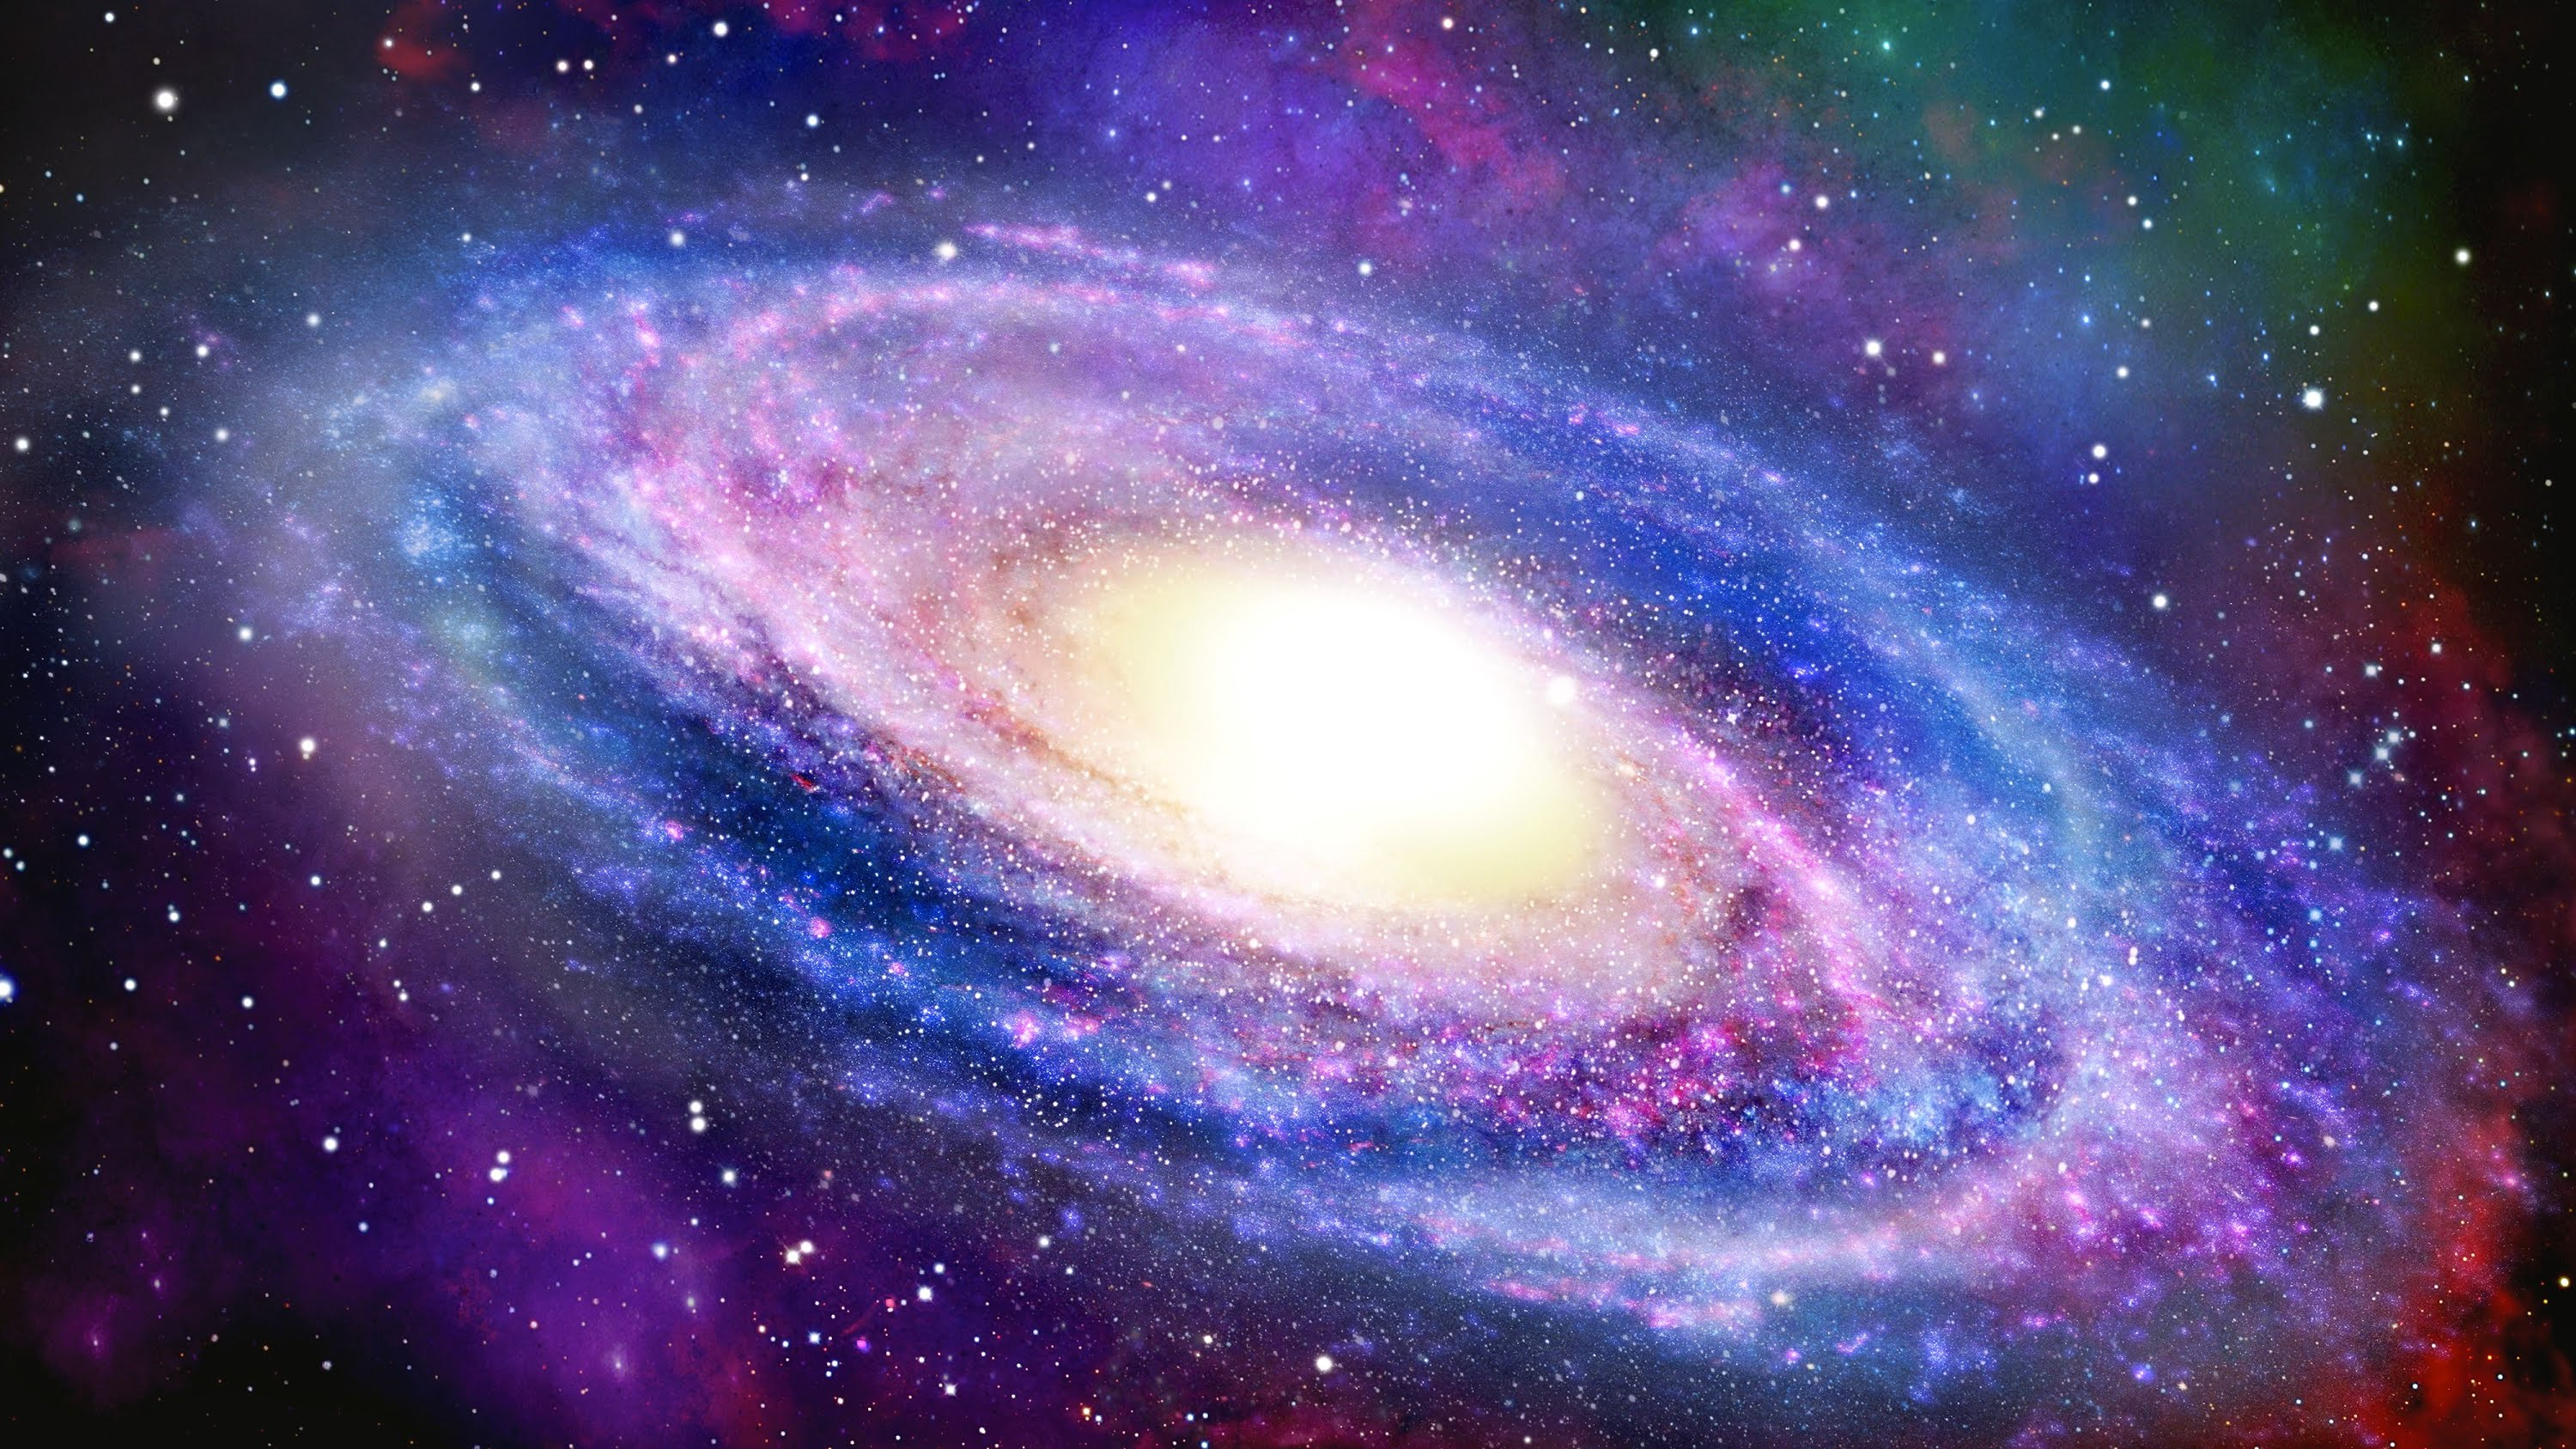
\includegraphics[scale=0.1]{universe}
	
		\caption{Sample picture of universe }
		\label{c6:fig1}
	\end{center}
	\end{figure}

There's a picture of a galaxy in Fig. \ref{c6:fig1}

\section{Graph}
Another example is given in Fig. \ref{c6:fig2}

	\begin{figure}[htb]
		\begin{center}
		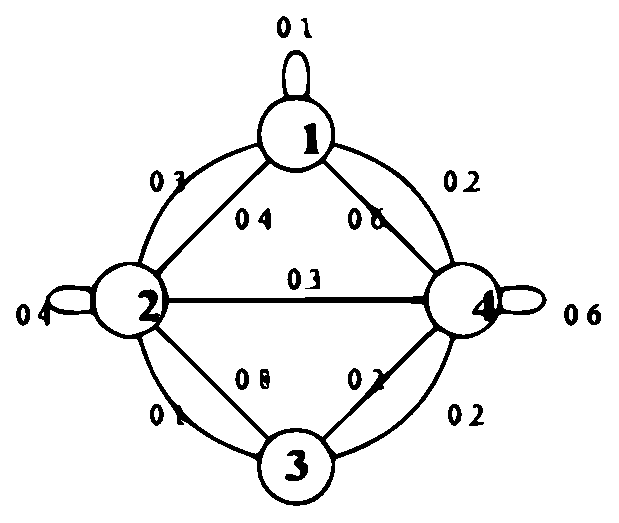
\includegraphics[scale=0.5]{graph}
	
		\caption{Sample graph }
		\label{c6:fig2}
	\end{center}
	\end{figure}



\chapter{CHAPTER TITLE} \label{c7}
\section{Conclusion}
This section will need to have several elements, including:
\begin{itemize}
	\item A brief summary, just a few paragraphs, of your key findings, related back to what you expected to see (essential);
	\item The conclusions which you have drawn from your research (essential);
	\item Why your research is important for researchers and practitioners (essential);
	\item Recommendations for future research (strongly recommended, verging on essential);
	\item Recommendations for practitioners (strongly recommended in management and business courses and some other areas, so check with your supervisor whether this will be expected); and a final paragraph rounding off your dissertation or thesis.
\end{itemize}




\end{spacing}
%\input{chapter8/chapter8-conclusion}
\addcontentsline{toc}{chapter}{\bf ~~~~~~~~~~~REFERENCES}
% \bibliographystyle{IEEEtran}
\bibliography{references/references}
\newpage 
\begin{spacing}{1.5}
\chapter*{\centering \large\textbf{LIST OF PUBLICATIONS RELEVANT TO THE THESIS}}
\addcontentsline{toc}{chapter}{\bf ~~~~~~~~~~~LIST OF PUBLICATIONS}
\noindent
\begin{enumerate}
	
\item Slavin, S. J., Schindler, D. L., \& Chibnall, J. T. (2014). Medical student mental health 3.0: improving student wellness through curricular changes. Academic Medicine, 89(4), 573-577.


\end{enumerate}
(List of publication should not contain communicated papers and under review
papers)
\end{spacing}


	\begin{appendices}
		\appendixpage
		\noappendicestocpagenum
		\addappheadtotoc
		\chapter{Sample Code}\label{app1}


\begin{lstlisting}
def calculate_area(shape, dimensions):
  """
  This function calculates the area of a shape based on its type and dimensions.

  Args:
      shape (str): The type of shape (e.g., "rectangle", "circle").
      dimensions (list): A list containing the shape's dimensions.

  Returns:
      float: The calculated area of the shape.
  """
  if shape == "rectangle":
    length, width = dimensions
    return length * width
  elif shape == "circle":
    radius = dimensions[0]
    return 3.14159 * radius ** 2
  else:
    print(f"Error: Unsupported shape '{shape}'.")
    return None

def analyze_text(text):
  """
  This function analyzes a text string and returns some basic statistics.

  Args:
      text (str): The text string to be analyzed.

  Returns:
      dict: A dictionary containing the number of words, characters, and uppercase letters.
  """
  words = len(text.split())
  chars = len(text)
  uppercase = sum(1 for char in text if char.isupper())
  return {"words": words, "characters": chars, "uppercase": uppercase}

def create_shopping_list(items, quantities=None):
  """
  This function creates a shopping list with items and optional quantities.

  Args:
      items (list): A list of items to include in the shopping list.
      quantities (list, optional): A list of corresponding quantities for each item. 

  Returns:
      str: The formatted shopping list string.
  """
  shopping_list = ""
  if quantities:
    for item, quantity in zip(items, quantities):
      shopping_list += f"- {quantity} {item}\n"
  else:
    for item in items:
      shopping_list += f"- {item}\n"
  return shopping_list.rstrip()

# Example usage
shapes = [("rectangle", [5, 3]), ("circle", [4])]
for shape, dimensions in shapes:
  area = calculate_area(shape, dimensions)
  if area:
    print(f"The area of the {shape} is: {area:.2f}")

text_data = analyze_text("This is a sample text string for analysis.")
print(f"The text contains: {text_data['words']} words, {text_data['characters']} characters, and {text_data['uppercase']} uppercase letters.")

shopping_items = ["Milk", "Bread", "Eggs", "Apples"]
shopping_list = create_shopping_list(shopping_items)
print("\nShopping List:")
print(shopping_list)
\end{lstlisting}
		%\chapter{'t' TABLE}\label{app2}
%\begin{figure}[H]
%	\centering
%	\includegraphics[scale=0.7]{./images/t-table}
%\end{figure}

\begin{table}[htb]
	
	\resizebox{\linewidth}{!}{
		\tiny
\begin{tabular}{ll|lllllllllllllllllll|ll}
	\multicolumn{2}{c|}{Tail}& \multicolumn{19}{c}{\bf Degrees of
		Freedom}&\multicolumn{2}{|c}{Confidence}\\
	\multicolumn{2}{c|}{Probability}&1&2&3&4&5&6&7&8&9&10&12&15&20&25&30&40&50&1
	
	00&1000&\multicolumn{2}{|c}{Levels}\\  
	1-tail&2-tail & & & & & & & & & & & & & & & & & & & $\approx \infty$
	&2-sided & 1-sided \\ \hline
	
	%Body of table begins here
	
	0.5 & 1&  0.000 &  0.000 &  0.000 &  0.000 &  0.000 &  0.000 &  0.000 & 
	0.000 &  0.000 &  0.000 &  0.000 &  0.000 &  0.000 &  0.000 &  0.000 & 
	0.000 &  0.000 &  0.000 &  0.000 && \\
	
	0.4 & 0.8 &  0.325 &  0.289 &  0.277 &  0.271 &  0.267 &  0.265 &  0.263 & 
	0.262 &  0.261 &  0.260 &  0.259 &  0.258 &  0.257 &  0.256 &  0.256 & 
	0.255 &  0.255 &  0.254 &  0.253 & &\\
	
	0.3 & 0.6 &  0.727 &  0.617 &  0.584 &  0.569 &  0.559 &  0.553 &  0.549 & 
	0.546 &  0.543 &  0.542 &  0.539 &  0.536 &  0.533 &  0.531 &  0.530 & 
	0.529 &  0.528 &  0.526 &  0.525 & &\\
	
	0.25 & 0.5&  1.000 &  0.816 &  0.765 &  0.741 &  0.727 &  0.718 &  0.711 & 
	0.706 &  0.703 &  0.700 &  0.695 &  0.691 &  0.687 &  0.684 &  0.683 & 
	0.681 &  0.679 &  0.677 &  0.675 && \\
	
	0.2 & 0.4& 1.376 &  1.061 &  0.978 &  0.941 &  0.920 &  0.906 &  0.896 & 
	0.889 &  0.883 &  0.879 &  0.873 &  0.866 &  0.860 &  0.856 &  0.854 & 
	0.851 &  0.849 &  0.845 &  0.842 &&80\%\\ \hline
	
	0.17 & 0.34&  1.691 &  1.242 &  1.132 &  1.082 &  1.054 &  1.036 &  1.024 &
	1.015 &  1.008 &  1.002 &  0.994 &  0.986 &  0.977 &  0.973 &  0.970 & 
	0.966 &  0.963 &  0.959 &  0.955 && \\
	
	0.15 & 0.3& 1.963 &  1.386 &  1.250 &  1.190 &  1.156 &  1.134 &  1.119 & 
	1.108 &  1.100 &  1.093 &  1.083 &  1.074 &  1.064 &  1.058 &  1.055 & 
	1.050 &  1.047 &  1.042 &  1.037 &  &\\
	
	0.14 & 0.28 & 2.125 &  1.467 &  1.315 &  1.248 &  1.211 &  1.187 &  1.171 &
	1.159 &  1.149 &  1.142 &  1.131 &  1.121 &  1.110 &  1.104 &  1.100 & 
	1.095 &  1.092 &  1.086 &  1.081& &  \\
	
	0.13 & 0.26 &  2.311 &  1.556 &  1.385 &  1.311 &  1.270 &  1.244 &  1.226
	&  1.212 &  1.202 &  1.194 &  1.182 &  1.171 &  1.159 &  1.153 &  1.148 & 
	1.143 &  1.139 &  1.133 &  1.127 &&\\
	
	0.12 & 0.24 & 2.526 &  1.654 &  1.462 &  1.379 &  1.333 &  1.304 &  1.284 &
	1.269 &  1.258 &  1.249 &  1.236 &  1.224 &  1.211 &  1.204 &  1.199 & 
	1.193 &  1.189 &  1.182 &  1.176 &&\\ \hline
	
	0.11 & 0.22 & 2.778 &  1.763 &  1.545 &  1.453 &  1.401 &  1.369 &  1.347 &
	1.331 &  1.318 &  1.308 &  1.294 &  1.280 &  1.266 &  1.258 &  1.253 & 
	1.246 &  1.242 &  1.234 &  1.227 &&\\
	
	0.1 & 0.2 &  3.078 &  1.886 &  1.638 &  1.533 &  1.476 &  1.440 &  1.415 & 
	1.397 &  1.383 &  1.372 &  1.356 &  1.341 &  1.325 &  1.316 &  1.310 & 
	1.303 &  1.299 &  1.290 &  1.282 &80\% & 90\%\\
	
	0.09 & 0.18 & 3.442 &  2.026 &  1.741 &  1.623 &  1.558 &  1.517 &  1.489 &
	1.469 &  1.454 &  1.442 &  1.424 &  1.406 &  1.389 &  1.379 &  1.373 & 
	1.365 &  1.360 &  1.350 &  1.342 &&\\
	
	0.08 & 0.16 & 3.895 &  2.189 &  1.859 &  1.723 &  1.649 &  1.603 &  1.572 &
	1.549 &  1.532 &  1.518 &  1.498 &  1.478 &  1.459 &  1.448 &  1.441 & 
	1.432 &  1.426 &  1.416 &  1.406 &&\\
	
	0.075 & 0.15 &  4.165 &  2.282 &  1.924 &  1.778 &  1.699 &  1.650 &  1.617
	&  1.592 &  1.574 &  1.559 &  1.538 &  1.517 &  1.497 &  1.485 &  1.477 & 
	1.468 &  1.462 &  1.451 &  1.441 &&\\ \hline
	
	0.07 & 0.14 &  4.474 &  2.383 &  1.995 &  1.838 &  1.753 &  1.700 &  1.664
	&  1.638 &  1.619 &  1.603 &  1.580 &  1.558 &  1.537 &  1.524 &  1.516 & 
	1.506 &  1.500 &  1.488 &  1.477&&\\
	
	0.065 & 0.13 & 4.829 &  2.495 &  2.072 &  1.902 &  1.810 &  1.754 &  1.715
	&  1.687 &  1.666 &  1.650 &  1.626 &  1.602 &  1.579 &  1.566 &  1.557 & 
	1.546 &  1.539 &  1.527 &  1.515&&\\
	
	0.06 & 0.12 &  5.242 &  2.620 &  2.156 &  1.971 &  1.873 &  1.812 &  1.770
	&  1.740 &  1.718 &  1.700 &  1.674 &  1.649 &  1.624 &  1.610 &  1.600 & 
	1.589 &  1.582 &  1.568 &  1.556 &&\\
	
	0.055 & 0.11 &  5.730 &  2.760 &  2.249 &  2.048 &  1.941 &  1.874 &  1.830
	&  1.797 &  1.773 &  1.754 &  1.726 &  1.699 &  1.672 &  1.657 &  1.647 & 
	1.635 &  1.627 &  1.613 &  1.600 &&\\
	
	0.05 & 0.1 & 6.314 &  2.920 &  2.353 &  2.132 &  2.015 &  1.943 &  1.895 & 
	1.860 &  1.833 &  1.812 &  1.782 &  1.753 &  1.725 &  1.708 &  1.697 & 
	1.684 &  1.676 &  1.660 &  1.646 & 90\% & 95\%\\  \hline
	
	0.045 & 0.09 & 7.026 &  3.104 &  2.471 &  2.226 &  2.098 &  2.019 &  1.966
	&  1.928 &  1.899 &  1.877 &  1.844 &  1.812 &  1.782 &  1.764 &  1.752 & 
	1.737 &  1.729 &  1.712 &  1.697 &&\\
	
	0.04 & 0.08 & 7.916 &  3.320 &  2.605 &  2.333 &  2.191 &  2.104 &  2.046 &
	2.004 &  1.973 &  1.948 &  1.912 &  1.878 &  1.844 &  1.825 &  1.812 & 
	1.796 &  1.787 &  1.769 &  1.752 &&\\
	
	0.035 & 0.07 & 9.058 &  3.578 &  2.763 &  2.456 &  2.297 &  2.201 &  2.136
	&  2.090 &  2.055 &  2.028 &  1.989 &  1.951 &  1.914 &  1.893 &  1.879 & 
	1.862 &  1.852 &  1.832 &  1.814&&\\
	
	0.03 & 0.06 & 10.57 &  3.896 &  2.951 &  2.601 &  2.422 &  2.313 &  2.241 &
	2.189 &  2.150 &  2.120 &  2.076 &  2.034 &  1.994 &  1.970 &  1.955 & 
	1.936 &  1.924 &  1.902 &  1.883 &&\\
	
	0.025 & 0.05 & 12.70 &  4.303 &  3.182 &  2.776 &  2.571 &  2.447 &  2.365
	&  2.306 &  2.262 &  2.228 &  2.179 &  2.131 &  2.086 &  2.060 &  2.042 & 
	2.021 &  2.009 &  1.984 &  1.962 &95\% & \\  \hline
	
	0.02 & 0.04 & 15.89 &  4.849 &  3.482 &  2.999 &  2.757 &  2.612 &  2.517 &
	2.449 &  2.398 &  2.359 &  2.303 &  2.249 &  2.197 &  2.167 &  2.147 & 
	2.123 &  2.109 &  2.081 &  2.056&&98\%\\
	
	0.017 & 0.034 & 18.71 &  5.284 &  3.712 &  3.166 &  2.895 &  2.734 &  2.628
	&  2.553 &  2.498 &  2.454 &  2.392 &  2.333 &  2.276 &  2.243 &  2.222 & 
	2.195 &  2.180 &  2.150 &  2.123&&\\
	
	0.015 & 0.03 & 21.21 &  5.643 &  3.896 &  3.298 &  3.003 &  2.829 &  2.715
	&  2.634 &  2.574 &  2.527 &  2.461 &  2.397 &  2.336 &  2.301 &  2.278 & 
	2.250 &  2.234 &  2.202 &  2.173 &&\\
	
	0.012 & 0.024 & 26.51 &  6.338 &  4.241 &  3.541 &  3.200 &  3.000 &  2.870
	&  2.778 &  2.710 &  2.658 &  2.582 &  2.511 &  2.442 &  2.403 &  2.378 & 
	2.346 &  2.328 &  2.292 &  2.261 &&\\
	
	0.01 & 0.02 & 31.82 &  6.965 &  4.541 &  3.747 &  3.365 &  3.143 &  2.998 &
	2.896 &  2.821 &  2.764 &  2.681 &  2.602 &  2.528 &  2.485 &  2.457 & 
	2.423 &  2.403 &  2.364 &  2.330 &98\%&99\%\\   \hline
	
	0.007 & 0.014 & 45.47 &  8.363 &  5.175 &  4.173 &  3.700 &  3.428 &  3.253
	&  3.131 &  3.041 &  2.972 &  2.873 &  2.781 &  2.693 &  2.642 &  2.610 & 
	2.570 &  2.547 &  2.501 &  2.462&&\\
	
	0.005 & 0.01 & 63.65 &  9.925 &  5.841 &  4.604 &  4.032 &  3.707 &  3.499
	&  3.355 &  3.250 &  3.169 &  3.055 &  2.947 &  2.845 &  2.787 &  2.750 & 
	2.704 &  2.678 &  2.626 &  2.581&99\%&99.5\%\\
	
	0.003 & 0.006 & 106.1 &  12.85 &  6.994 &  5.321 &  4.570 &  4.152 &  3.887
	&  3.705 &  3.573 &  3.472 &  3.330 &  3.197 &  3.073 &  3.003 &  2.957 & 
	2.902 &  2.870 &  2.808 &  2.754&&\\
	
	0.002 &  0.004 & 159.2 &  15.76 &  8.053 &  5.951 &  5.030 &  4.524 & 
	4.207 &  3.991 &  3.835 &  3.716 &  3.550 &  3.395 &  3.251 &  3.170 & 
	3.118 &  3.055 &  3.018 &  2.946 &  2.885&&\\
	
	0.001 &  0.002 & 318.3 &  22.32 &  10.21 &  7.173 &  5.893 &  5.208 & 
	4.785 &  4.501 &  4.297 &  4.144 &  3.930 &  3.733 &  3.552 &  3.450 & 
	3.385 &  3.307 &  3.261 &  3.174 &  3.098&99.8\%&99.9\%\\ \hline
	
	.0005 & 0.001 & 636.6 & 31.59 & 12.92 & 8.610 & 6.869 & 5.959 & 5.408 &
	5.041 & 4.781 & 4.587 & 4.318 & 4.073 & 3.850 & 3.725 & 3.646 & 3.551 &
	3.496 & 3.391 & 3.300 & 99.9\% & 99.95\%\\
	
	.0001 & .0002 & 3183  &  70.70 &  22.20 &  13.03 &  9.678 &  8.025 & 
	7.063
	&  6.442 &  6.010 &  5.694 &  5.263 &  4.880 &  4.539 &  4.352 &  4.234 & 
	4.094 &  4.014 &  3.862 &  3.733 &  &99.99\%\\
	
	5e-5 & .0001 & 6366 & 99.98 & 27.99 & 15.54 & 11.18 & 9.082 & 7.884 & 7.120
	& 6.594 & 6.210 & 5.694 & 5.239 & 4.837 & 4.620 & 4.482 & 4.320 & 4.228 &
	4.053 & 3.906 &99.99\% 
	
	%end of body of table
	
\end{tabular}}

\end{table}

\tiny{
	Courtesy: Robert J. MacG. Dawson $\star$ Dept.of Math \& Computing Science $\star$
	St. Mary's University, Halifax, NS, Canada B3H 3C3 $\star$ {\tt
		rdawson@husky1.stmarys.ca}}
	\end{appendices}
\end{document}
